\section{Results}
\label{results}

In section~\ref{methodology}, we discussed our sources, the sampling approach for Pythonic Idioms, and the JavaScript coding style guide. 
We then discussed how the input for Copilot to trigger code suggestions is restricted to ensure Copilot is deciding to suggest the desired way or vice-versa.
Finally, we discussed the evaluation method used to compare Copilot's code suggestions to the idiomatic approaches and the best practices listed in the coding style guide~(section~\ref{evaluation}).

In this section, we show the results of the study comparing Copilot suggestions against Pythonic idioms~(section~\ref{idioms}) addressing \textbf{RQ-1.1} (How do \cct{} manage programming idioms?) and JavaScript coding style guide~(section~\ref{smells}) addressing \textbf{RQ-1.2} (How do \cct{} manage manage to suggest non-smelly code?).

\section{Results}
\label{secidioms}
Using the methodology described in section~\ref{methodology}, we picked the top 10 most popular python idioms from work of Alexandru et al.~\cite{Alexandru2018} and compared Copilot suggestions when prompted with a input method~(shown in section~\ref{input}) and evaluated using methodology shown in section~\ref{evaluation}. 

Copilot suggested the idiomatic approach as the first suggestion in 2 of the 10 idioms we tested i.e., 2 out of 10 instances Copilot had the recommended way as its top suggestion. However, 4 out of those remaining 8 Idioms had the idiomatic way in Copilot's top 10 suggestions. Copilot did not have the idiomatic way in any of its top 10 suggestions for 4 idioms out of 10 idioms we tested.

Table~\ref{tab:all_idioms} shows the list of all the 10 idioms we tested and the ranking of the idiomatic way in Copilot suggestions (if it exists).

\renewcommand{\arraystretch}{1.7}
\begin{table}[ht]
    \centering
    \begin{tabular}{|L|c|}
    \hline
         \textbf{Idiom Title} & \textbf{Copilot Suggestion Matched?} \\
         & (out of 10 suggestions) \\
         \hline
         List comprehension & No \\
         \hline
         Dictionary comprehension & No \\
         \hline
         Mapping & 9\textsuperscript{th} \\
         \hline
         Filter &  7\textsuperscript{th} \\
         \hline
         Reduce & 9\textsuperscript{th} \\
         \hline
         List enumeration & No \\
         \hline
         Set comprehension & 1\textsuperscript{th} \\
         \hline
         Read and print from a file & 5\textsuperscript{th} \\
         \hline
         Add int to all list numbers & No \\
         \hline
         If condition check value & 1\textsuperscript{th} \\
         \hline
    \end{tabular}
    \caption{List of all python idioms tested on Copilot.}
    \label{tab:all_idioms}
\end{table}


Figure~\ref{fig:idioms_1} shows the example of list comprehension idiom, showing user input (i.e., human input), the top suggestion by Copilot and the idiomatic way from Alexandru et al.~\cite{Alexandru2018}.

\begin{figure}[hbt!]
    \centering
    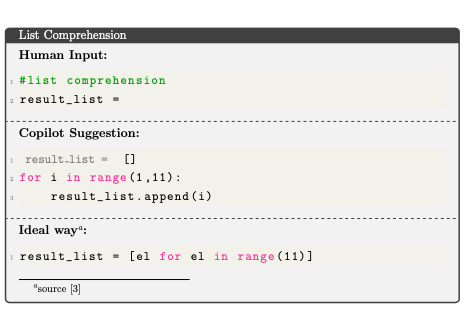
\includegraphics[width=\linewidth]{Figures/idioms_1.png}
    \caption{List Comprehension Idiom and Copilot Suggestion}
    \label{fig:idioms_1}
\end{figure}

The results show that Copilot did not suggest the optimal way as its first suggestion in the majority of the idioms we tested. This shows that current \cct{} like Copilot cannot suggest the idiomatic way in every suggestion even though they are the top most frequently used python idioms in public repositories on GitHub~\cite{Alexandru2018}. 

Copilot being closed source we cannot investigate the potential reasons behind this behavior. However, one plausible explanation for this behavior is that idiomatic ways may not be as frequent as non-idiomatic ways in Copilot's training data of public repositories on GitHub, making the non-idiomatic way rank higher than the idiomatic way.

\cct{} like Copilot should learn to detect idiomatic ways in public repositories and rank them higher than the most frequently used way in public repositories, so that the first suggestion would be the idiomatic way rather than the non-idiomatic way, which is the desirable way for \cct{} like Copilot. For the scope of this thesis, we leave resolving this problem as future work.

% \begin{tcolorbox}[title=List Comprehension,boxsep=.25mm]
%     %https://tex.stackexchange.com/questions/337909/tcolorbox-tcbline-style
% \textbf{Human Input:}
% \begin{lstlisting}[language={Python}]
% #list comprehension
% result_list = 
% \end{lstlisting}
% \tcbline
% \textbf{Copilot Suggestion:}
% \begin{lstlisting}[language=Python,escapechar=\%]
% % \noindent\textcolor{gray}{result\_list  =} % []
% for i in range(1,11):
%     result_list.append(i)
% \end{lstlisting}
% \tcbline
% \textbf{Idiomatic way\footnote{source \cite{Alexandru2018}}:}
% \begin{lstlisting}[language=Python]
% result_list = [el for el in range(11)]
% \end{lstlisting}
% \end{tcolorbox}

%%%%%% TODO: remember to update the screenshot if the source citation is different from the citation in the text %%%%%%

All the Idioms shown in Table~\ref{tab:all_idioms} can be found in the \repl{} including the code used as input (i.e., human input), the top suggestion by Copilot and the idiomatic way suggested in Alexandru et al.~\cite{Alexandru2018}.

\subsection{Code Smells}
\label{smells}
Using the methodology described in section~\ref{smells:methodology}, we sampled 10 best practices in javascript from AirBNB javascript coding style guide~\cite{airbnb_code} and compared Copilot syggestions when prompted with a input method(shown in section~\ref{smells:input}) and evaluated using methodology shown in section~\ref{smells:evaluation}. 

Copilot suggested the best practice from the coding guide for only one out of the ten coding standards we tested, i.e, 1 out of 10 instances Copilot had the recommended way as its top suggestion. Moreover, only 2 out of remaining 9 standards had the best practice in Copilot top 10 suggestions currently viewable. Copilot did not have the best practice in any of its top 10 suggestions for 7 standards out of 10 coding standards we tested.

% Copilot performed significantly worse than the Pythonic Idioms we showed in Section~\ref{secidioms}, As Copilot is closed source, we cannot find the reason behind this but one could argue that lack of data for JavaScript compared to python could be a reason for this behaviour. 

Table~\ref{tab:all_bp} shows the complete list of all the coding standards we tested on Copilot sampled from the AirBNB Coding Style guide~\cite{airbnb_code} and the ranking of the best practice in Copilot suggestions (if it exists).

\begin{table}[ht]
    \centering
    \begin{tabular}{|L|c|}
    \hline
         \textbf{Best Practice  Title} & \textbf{Copilot Suggestion Matched?} \\
         & (out of 10 suggestions) \\
         \hline
         Usage of Object method shorthand & No \\
         \hline
         Array Creating Constructor & 6\textsuperscript{th} \\
         \hline
         Copying Array Contents  & No \\
         \hline
         Logging a Function &  No \\
         \hline
         Exporting a Function & No \\
         \hline
         Sum of Numbers & 9\textsuperscript{th} \\
         \hline
         Accessing Properties & 1\textsuperscript{th} \\
         \hline
         Switch case usage & No \\
         \hline
         Return value from Function with a condition check & No \\
         \hline
         Converting Array-like object to an Array  & No \\
         \hline
    \end{tabular}
    \caption{List of all JavaScript Best Practices tested on Copilot.}
    \label{tab:all_bp}
\end{table}

Figure~\ref{fig:bp_1} shows the Best Practice for Copying Array Contents, showing user input (i.e., Human Input), the top suggestion by Copilot and the recommended way suggested by AirBNB JavaScript coding style guide~\cite{airbnb_code}.

\begin{figure}[hbt!]
    \centering
    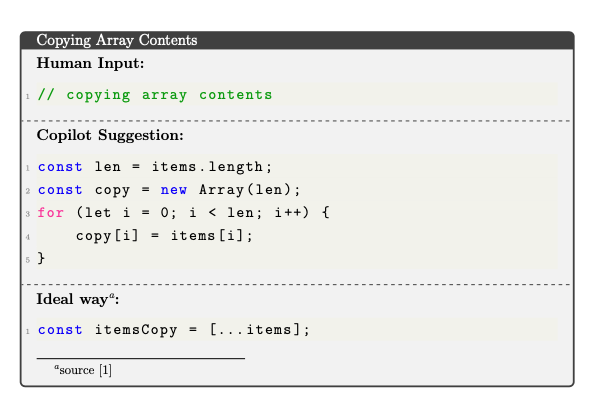
\includegraphics[width=\linewidth]{Figures/bp_1.png}
    \caption{Best Practice for Copying Array Contents and Copilot Suggestion.}
    \label{fig:bp_1}
\end{figure}

The results show that Copilot performed worse than the language idioms~(shown in chapter~\ref{chapter:idioms}). Copilot did not suggest the best practice as its first suggestion for 7 out of 10 coding standards we tested. This shows that current AI-supported
code completion tools like Copilot cannot suggest coding standards in its suggestions even though the coding standards are the sampled from widely accepted coding style guide.

All the Best Practices shown in Table~\ref{tab:all_bp} can be found in the \repl{} including the code used as input (i.e., human input), the top suggestion by Copilot and the best practice from AirBNB JavaScript coding style guide~\cite{airbnb_code}.

There could be many reasons for this performance like the public repositories do not always follow coding standards, Copilot cannot detect coding style from repositories that have contribution guides including the coding standards followed in the project. 
Copilot being closed source we cannot investigate the potential reasons behind this behavior and recommend ways to fix this issue improving the performance of Copilot.

We did not test Copilot for suggesting project specific coding styles because Copilot does not have the feature to customise its suggestions based on preferences~\cite{Copilot-web}.
However, \cct{} like Copilot should follow coding style guides and adapt their code suggestions to match the coding style used in the project. 
For example, if a user is working on a project where one of the coding style guideline says to leave a blank line after blocks and before the next statement~\cite{airbnb_code}. As a productivity tool, the ideal behaviour for \cct{} like Copilot is to detect the coding style guideline from existing code in the project and always suggest code that follows the guideline. 

% \begin{tcolorbox}[title=Copying Array Contents,boxsep=.15mm]
%     %https://tex.stackexchange.com/questions/337909/tcolorbox-tcbline-style
% \textbf{Human Input:}
% \begin{lstlisting}[language=JavaScript]
% // copying array contents
% \end{lstlisting}
% \tcbline
% \textbf{Copilot Suggestion:}
% \begin{lstlisting}[language=JavaScript]
% const len = items.length;
% const copy = new Array(len);
% for (let i = 0; i < len; i++) {
% 	  copy[i] = items[i];
% }
% \end{lstlisting}
% \tcbline
% \textbf{Ideal way\footnote{source \cite{airbnb_code}}:}
% \begin{lstlisting}[language=JavaScript]
% const itemsCopy = [...items];
% \end{lstlisting}
% \end{tcolorbox}

%%%%%% TODO: remember to update the screenshot if the source citation is different from the citation in the text %%%%%%


\subsection{Summary of Findings}
In an attempt to find the boundaries of \cct{} like Copilot, we analyzed Copilot code suggestions for Pythonic idioms and JavaScript best practices. 
We identified that Copilot did not suggest the idiomatic way as its top suggestion for 23 out of 25 coding scenarios in Python. 
Furthermore, we identified that Copilot did not suggest the recommended best practice for 22 out of 25 coding scenarios in JavaScript.

Although Copilot is very good at solving well-specified programming contest style problems~\cite{empirical_eval}, our experiments show that it does not do well in following idioms and recommending best practices in its code suggestions.
Additionally, \cct{} like Copilot being a productivity tool, should be able to suggest idiomatic approaches and recommended best practices in its code suggestions to be helpful for the user.
Studies like ours might help use this delineation to understand what might help turn \cct{} such as Copilot into full-fledged \AISE{} tools.
\section{Chapter Summary}
In summary, we start this chapter by showing the methodology used in addressing textbf{RQ-1} (What are the current boundaries of \cct{}?). 
We first introduced Pythonic idioms and best practices in JavaScript.
We then present our sampling approach for sampling 25 coding scenarios to analyze Copilot code suggestions.
Furthermore, we discussed the input given to Copilot to trigger a code suggestion 
and how the input was restricted to deriving the desired way from the input.
Finally, we described our evaluation approach for Copilot code suggestions.

We sampled 25 Pythonic idioms from Alexandru et al.~\cite{Alexandru2018}, and Farook et al.~\cite{idioms}.
We identified that Copilot did not suggest the idiomatic way as its top suggestion for 23 out of 25 coding scenarios in Python, which addressed \textbf{RQ-1.1} (How do \cct{} manage programming idioms?).
Furthermore, we sampled 25 best practices in JavaScript from the AirBNB JavaScript coding style guide~\cite{airbnb_code}. We identified that Copilot did not suggest the recommended best practice for 22 out of 25 coding scenarios in JavaScript, which addressed \textbf{RQ-1.2} (How do \cct{} manage to manage to suggest non-smelly code?).


% we showed that Copilot struggles to detect and most common idiomatic ways present in public repositories of GitHub and rank them higher than the non-idiomatic ways. The ideal behavior of \cct{} like Copilot in solving this problem is detecting common patterns present in code and rank them higher as the idiomatic ways for a task.
% In the next chapter (chapter~\ref{smells}), we look into how this ideal behavior can cause problems in the case of code smells, where common bad practices present in public repositories of GitHub can make \cct{} like Copilot introduce bad coding practices in its suggestions.

% % \section{Chapter Summary}
% In summary, we start this chapter by showing the methodology used in addressing \textbf{RQ-1.2} (How do \cct{} manage to suggest non-smelly code?). We first introduced the study setup with the input to Copilot and how it was restricted to deriving the best practice from the input and how the suggestions from Copilot were evaluated. We sampled best practices from AirBNB JavaScript coding style guide~\cite{airbnb_code}, and then compared it against Copilot suggestions. Based on results shown in Table~\ref{tab:all_bp}, Copilot struggles to suggest the best practices from widely used coding standards in its suggestions. 

In this chapter, we showed that Copilot struggles to detect and follow coding style guides present in public repositories of GitHub and always suggests code that follows those coding style guides. We also observed that Copilot struggles to detect and most common idiomatic ways present in public repositories of GitHub and rank them higher than the non-idiomatic ways. 
Identifying this delineation could help in urn AI-supported code completion tools such as Copilot into full-fledged AI-supported software engineering tools.
In the next chapter (chapter~\ref{chapter:framework}), we illustrate our taxonomy inspired by autonomous driving levels on the software abstraction hierarchy in \AISE{} and delineate where \cct{} like Copilot currently stands in the taxonomy. 